\appendix


%%%%%%%%%%%%%%%%%%%%%%%%%%%%%%%%%%%%%%%%%%%%%%%%%%%%%%%%%%%%%%%%%%%%%%
%%%%%%%%%%%%%%%% Convolutional Networks for Semantic Segmentation
%%%%%%%%%%%%%%%%%%%%%%%%%%%%%%%%%%%%%%%%%%%%%%%%%%%%%%%%%%%%%%%%%%%%%%

\section{Convolutional Networks for Semantic Segmentation}
\subsection{Convolutional Neural Networks}

A Convolutional Neural Network (CNN) for image processing is often comprised of stacked convolutional layers with interlacing subsampling layers for feature extraction, followed by a few task-specific layers.% for either classification or regression.
For instance, fully connected layers are often used for object recognition\cite{lecun1998gradient,krizhevsky2012imagenet}, region proposal\cite{ren2015faster}, etc., and transposed convolutions or dilated convolutions together with convolutional layers can be used for semantic segmentation\cite{long2015fully,yu2015multi}.

An example, LeNet-5 (1998) \cite{lecun1998gradient}, is shown in Figure \ref{fig:lenet}.
The first convolutional layer of LeNet contains 6 convolutional kernels of size 5x5 and each convolutional kernels convolve with small windows sliding over the images and produce a feature map of size 28x28.
Each output in the produced feature map is corresponding to a small sub-region of the visual field (the image), called a \textit{receptive field}.
A following max pooling layer subsamples the feature maps by a factor of two by extracting the maximum values for every two adjacent pixels literally and vertically.
The result feature map S2 has a shape of 14 by 14 and a receptive field of 6 by 6.
Another sequence of convolutional and pooling layers generate feature maps of size 5x5 with receptive field 16x16.
Neurons in the last three layers of LeNet are fully connected to the layer before and the layer after if exists, creating the final prediction for 10 classes.

The bottom layers in the convolutional layer stack have smaller receptive fields while the top layers have larger receptive fields.
A small receptive field means that the filter have access to information only in a local sub-region of the image while a large receptive field can convey more global information.
This trend of varying pattern responses from local to global, from simple to complex for stacked convolutional layers is a reflect of emulating animals visual cortex.
In cat's visual cortex\cite{hubel1962receptive}, two basic cell types of visual cortex have been identified:
Simple cells respond maximally to specific edge-like patterns within their receptive field.
Complex cells have larger receptive fields and are locally invariant to the exact position of the pattern.
The shallower convolutional layers play a similar functionlity as simple cells while the deeper layers maps are similar to complex cells.

%%%%%%%% FIGURE LeNet
\begin{figure}[t]
\centering
   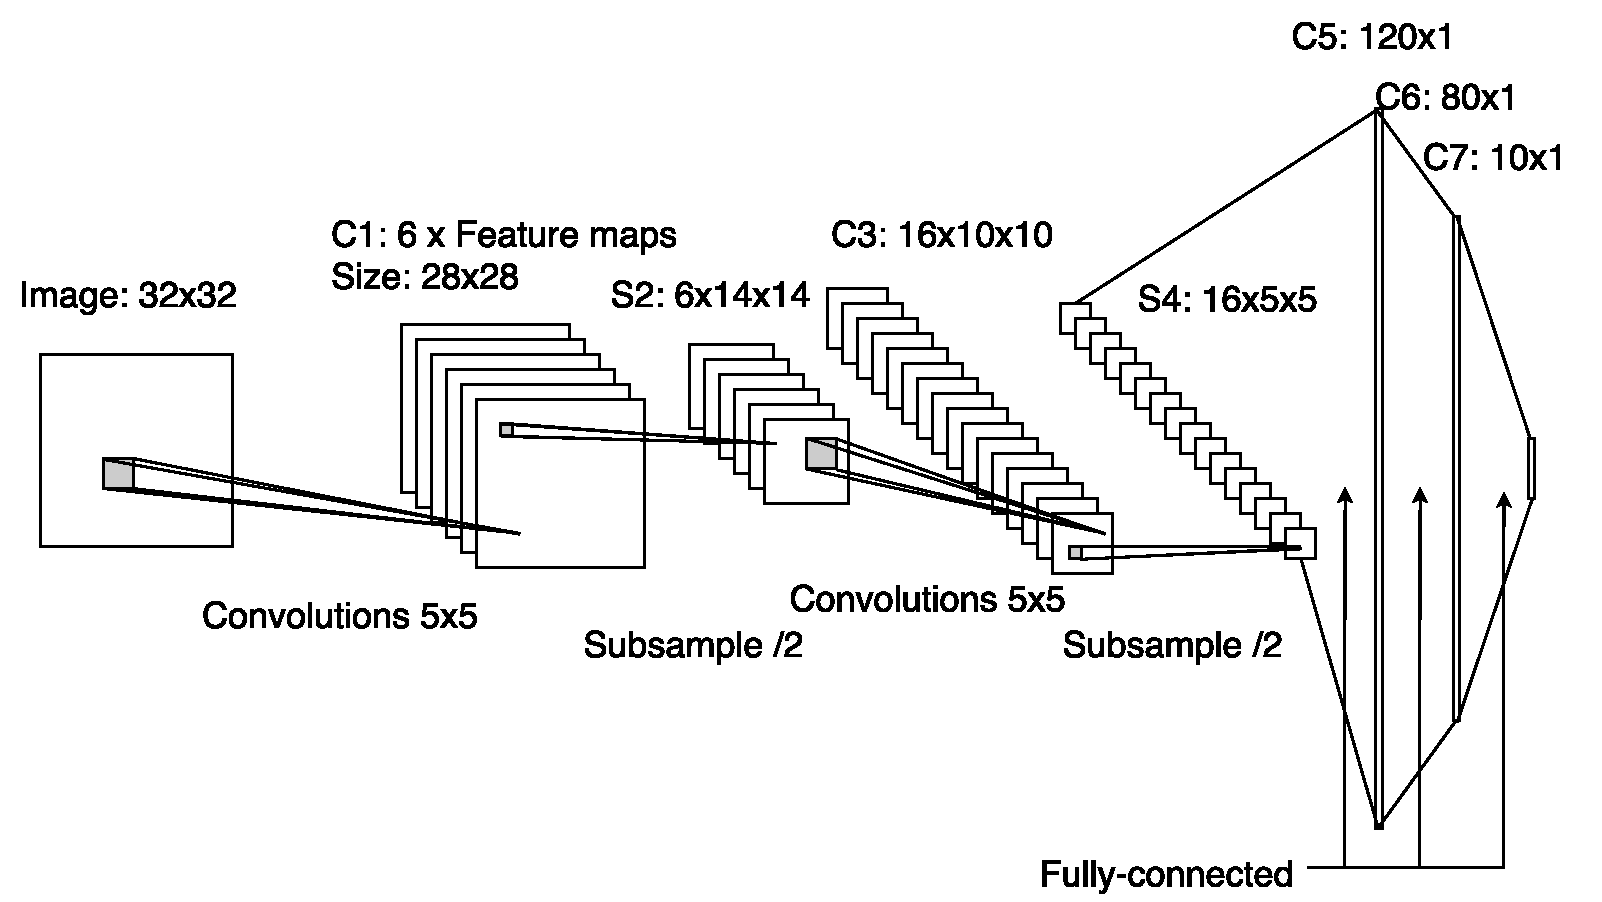
\includegraphics[width=\linewidth]{img/lenet}
\caption{An example convolutional neural network, LeNet-5\cite{lecun1998gradient}}
\label{fig:lenet}
\end{figure}

The main benefit of CNN compared to the traditional multilayer perceptron is that it is easier to optimize due to the local connectivy pattern of convolutional layers and spatial weights sharing.
Because of the design choice of convolutional neurons and maximum pooling, translation invariance as well as scaling invariance and distortion invariance to some extent are achievable for convolutional neural networks.\cite{lecun1998gradient}
Different from the traditional handcrafted features, learnable convolutional features normally generalize well and can achieve better performance for dataset with a complex input distribution.\cite{krizhevsky2012imagenet}
By increasing the number of convolution layers and number of filters in each layer, one can create CNN models with high capacity, meaning a large space of representable functions.
This can be beneficial for datasets of immense complexity, for example, ILSVRC\cite{russakovsky2015imagenet}, Microsoft COCO\cite{lin2014microsoft}, as long as there are sufficient training samples with an appropriate optimization strategy.


\subsection{Semantic image segmentation}

Semantic image segmentation is to segment images into semantically meaningful partitions, a.k.a.,\textit{segments}.
It can be operated as classifying pixels into the corresponding pre-defined categories.
The success of CNN models on object classification tasks can be extended for semantic image segmentation tasks.\cite{long2015fully}
As we discussed in the previous session, convolutional layers can extract hierarchical features, which from low-level to high-level encode information from local to global.
In contrast to object classification tasks, which normally only need global information to resolve semantics, segmentation tasks also require local information to resolve locations.
One of the primary difficulties of applying CNN model to segmentation tasks is how to combine global information and local information to solve semantics and locations altogether.
Long et al.\cite{long2015fully} proposed a so-called skip architecture to aggregate information from the local low-level features in the hierarchy with global information from the high-level features.
The low-level features are fine, presenting appearances and the high-level features are coarse, revealing semantics.
By combining them together, it becomes possible to create accurate and detailed segmentation.
% in an end-to-end, pixel-by-pixel fully convolutional neural networks for semantic segmentation.%%%%%%%% FIGURE LeNet

\begin{figure}[t]
\centering
   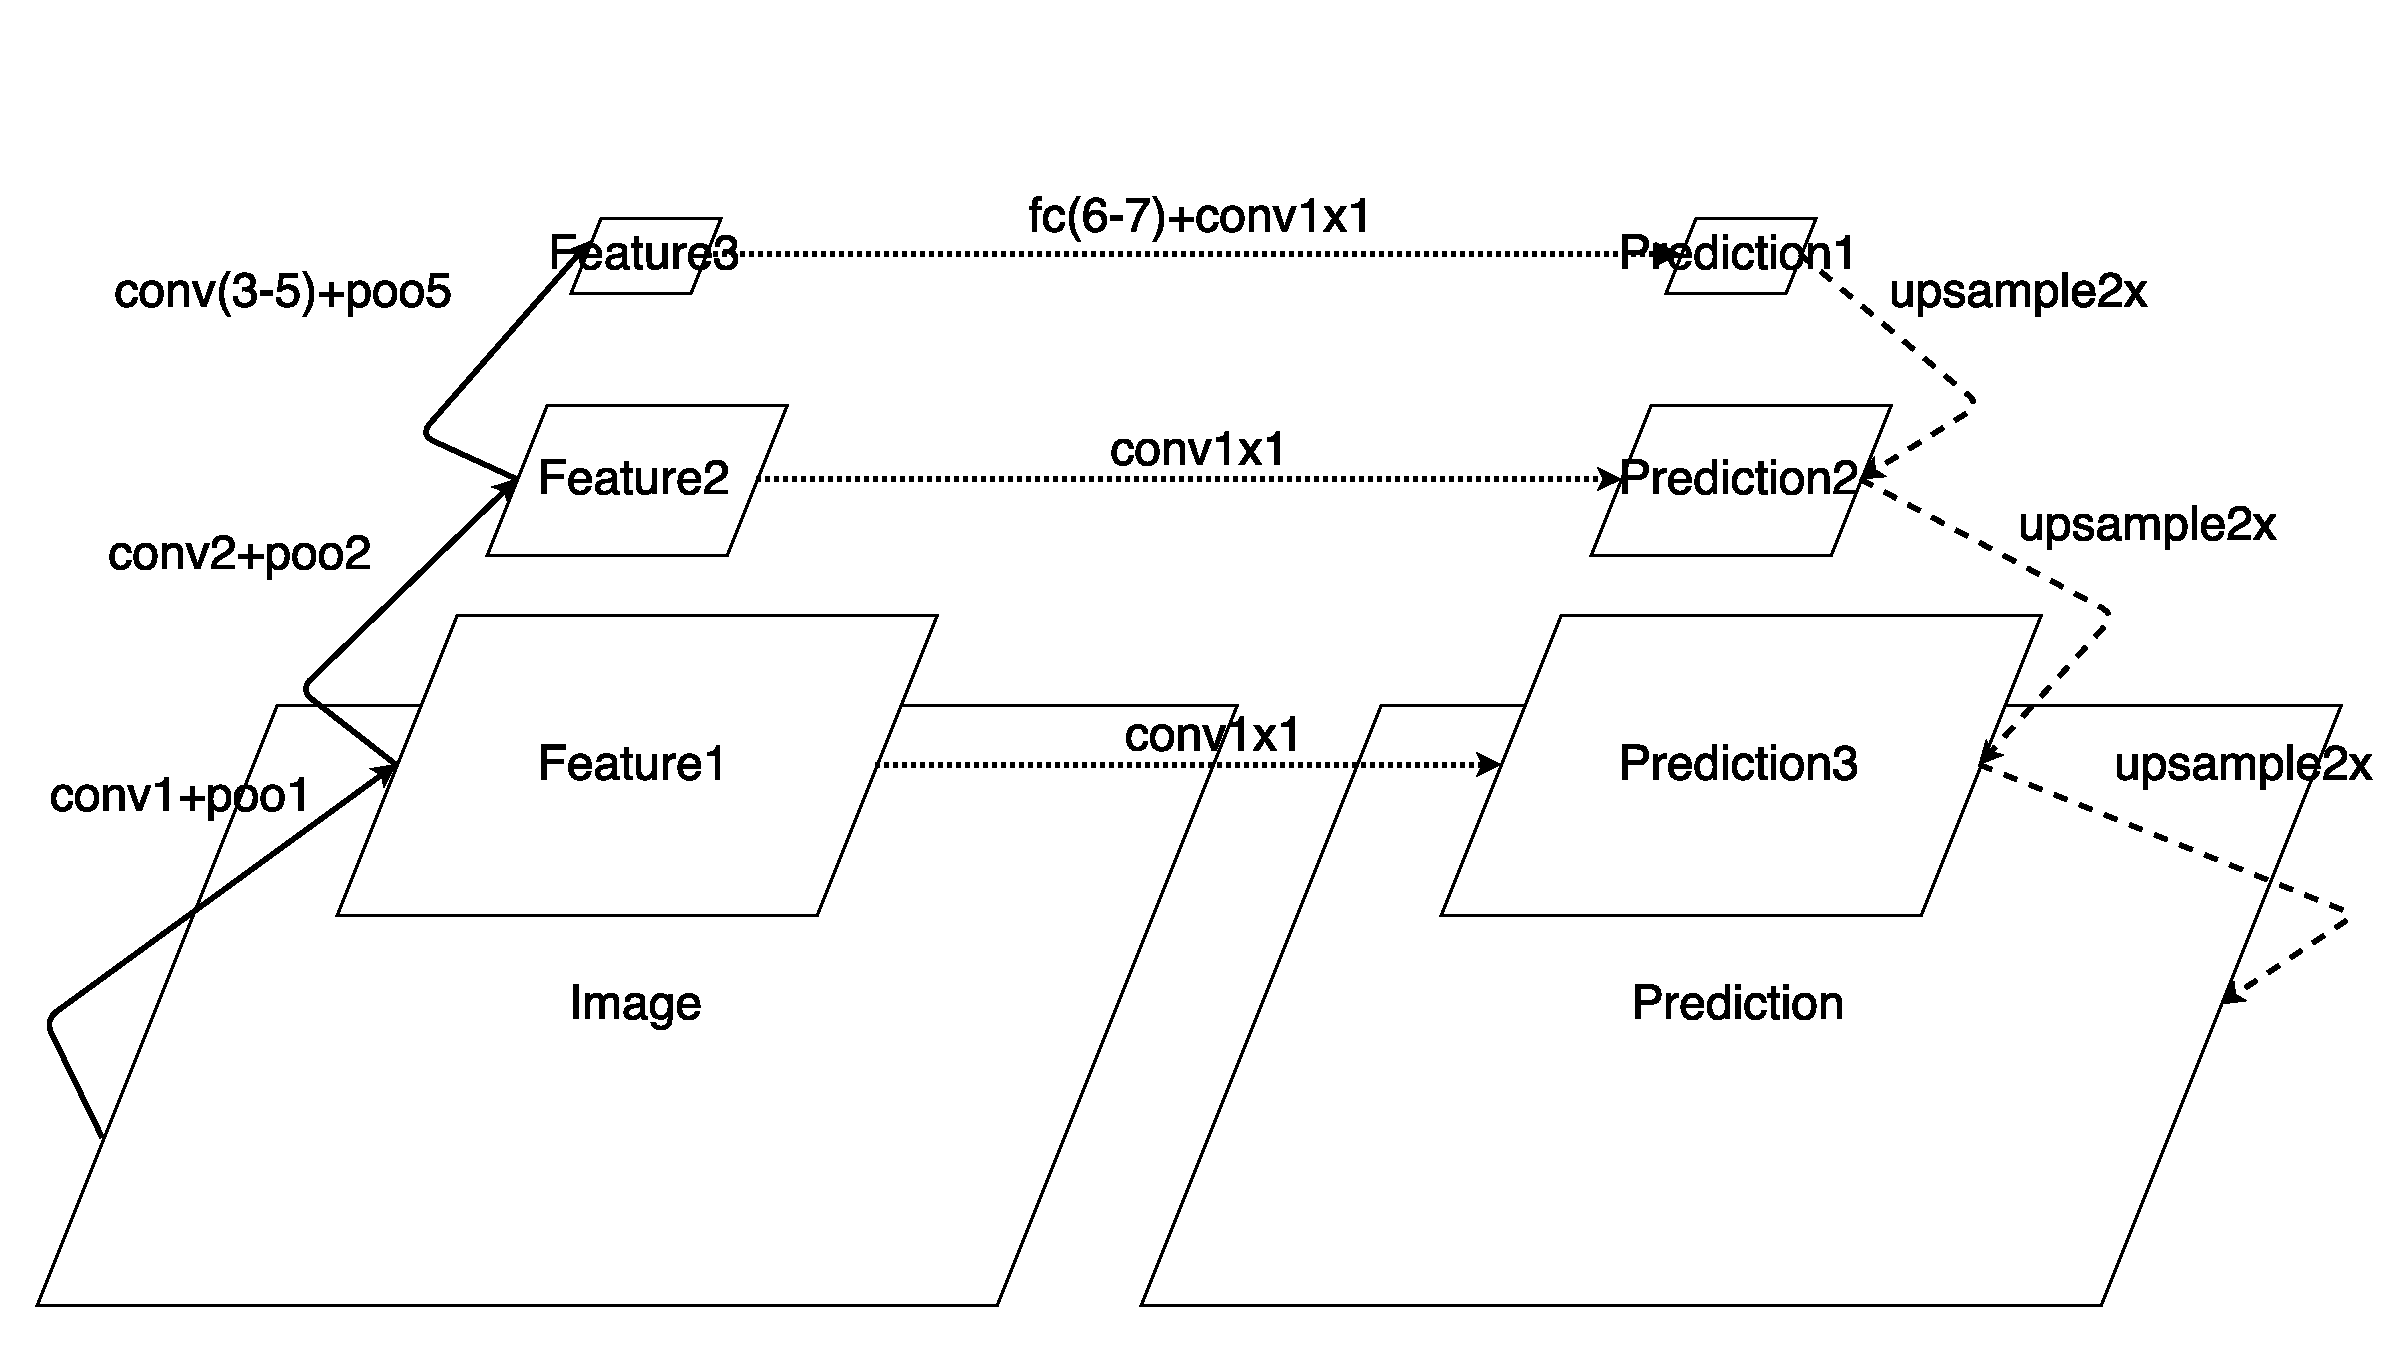
\includegraphics[width=\linewidth]{img/fcn}
\caption{Fully convolutional network (FCN) by Long et al. (2015) \cite{long2015fully}.}
\label{fig:fcn}
\end{figure}

Figure \ref{fig:fcn} shows the architecture of so-called fully convolutional networks (FCN) by Long et al. (2015).

\subsection{Transferring convolutional neural nets}

%%%%%%%%%%%%%%%%%%%%%%%%%%%%%%%%%%%%%%%%%%%%%%%%%%%%%%%%%%%%%%%%%%%%%%
%%%%%%%%%%%%%%%% Deep Learning with label noise
%%%%%%%%%%%%%%%%%%%%%%%%%%%%%%%%%%%%%%%%%%%%%%%%%%%%%%%%%%%%%%%%%%%%%%

\section{Deep Learning with Label Noise}
\subsection{Learning in the presence of label noise}

NNAR, NAR, NCAR

Such a noise model is called noisy not at random (NNAR) \cite{frenay2014classification} because the noise depends on not only the true label $y$ but also the inputs $x$.

\subsection{Deep learning models robust to label noise}


%%%%%%%%%%%%%%%%%%%%%%%%%%%%%%%%%%%%%%%%%%%%%%%%%%%%%%%%%%%%%%%%%%%%%%
%%%%%%%%%%%%%%%% Supportive information
%%%%%%%%%%%%%%%%%%%%%%%%%%%%%%%%%%%%%%%%%%%%%%%%%%%%%%%%%%%%%%%%%%%%%%
\section{Supportive information}
\label{sec:support}

\subsection{An 8-layer Convolutional neural network}


% Please add the following required packages to your document preamble:
%%%%%%%% Table 8-layer CNN
\begin{table}[t]
\resizebox{\columnwidth}{!}{
\centering
\begin{tabular}{c|c|c}
\hline
layer name             & output size                     & 8-layer                               \\ \hline
\multirow{3}{*}{conv1} & \multirow{3}{*}{16 $\times$ 16} & 3 $\times$ 3, 32, LeakyReLU(0.2)      \\ \cline{3-3}
                       &                                 & 3 $\times$ 3, 32, LeakyReLU(0.2)      \\ \cline{3-3}
                       &                                 & 2 $\times$ 2 max pool, dropout(0.2)   \\ \hline
\multirow{3}{*}{conv2} & \multirow{3}{*}{8 $\times$ 8}   & 3 $\times$ 3, 64, LeakyReLU(0.2)      \\ \cline{3-3}
                       &                                 & 3 $\times$ 3, 64, LeakyReLU(0.2)      \\ \cline{3-3}
                       &                                 & 2 $\times$ 2 max pool, dropout(0.2)   \\ \hline
\multirow{3}{*}{conv3} & \multirow{3}{*}{4 $\times$ 4}   & 3 $\times$ 3, 128, LeakyReLU(0.2)     \\ \cline{3-3}
                       &                                 & 3 $\times$ 3, 128, LeakyReLU(0.2)     \\ \cline{3-3}
                       &                                 & 2 $\times$ 2 max pool, dropout(0.2)   \\ \hline
\multirow{2}{*}{fc}    & \multirow{2}{*}{1 $\times$ 1}   & flatten, 512-d fc, ReLU, dropout(0.5) \\ \cline{3-3}
                       &                                 & 11-d fc, softmax                      \\ \hline
\multicolumn{2}{c|}{Parameters}                          & 1,341,739                             \\ \hline
\end{tabular}
}
\caption{8-layer Convolutional Neural Networks used for the CIFAR dataset classification.}
\label{fig:8layer}
\end{table}

\subsection{Evaluation metrics}

(overall) accuracy
$$ \text{accuracy} = \frac{\text{true pos. + true neg.}}{\text{true pos. + false pos. + true neg. + false neg.}}$$

precision
$$\text{precision} = \frac{\text{true pos.}}{\text{true pos. + false pos.}}$$

recall
$$\text{recall} = \frac{\text{true pos.}}{\text{true pos. + false neg.}}$$

f1-score
$$F_1 = 2 \cdot \frac{\text{precision} \cdot \text{recall}}{\text{precision}+\text{recall}}$$

intersection over union (IU)
$$ \text{IU} = \frac{\text{true pos.}}{\text{true pos. + false pos. + false neg.}}$$

%%%%%%%%%%%%%%%%%%%%%%%%%%%%%%%%%%%%%%%%%%%%%%%%%%%%%%%%%%%%%%%%%%%%%%
%%%%%%%%%%%%%%%% Appendix Results                     %%%%%%%%%%%%%%%%
%%%%%%%%%%%%%%%%%%%%%%%%%%%%%%%%%%%%%%%%%%%%%%%%%%%%%%%%%%%%%%%%%%%%%%

\section{Additional Results}

%%%%%%%% FIGURE Number of training categories
\begin{figure}[t]
\centering
   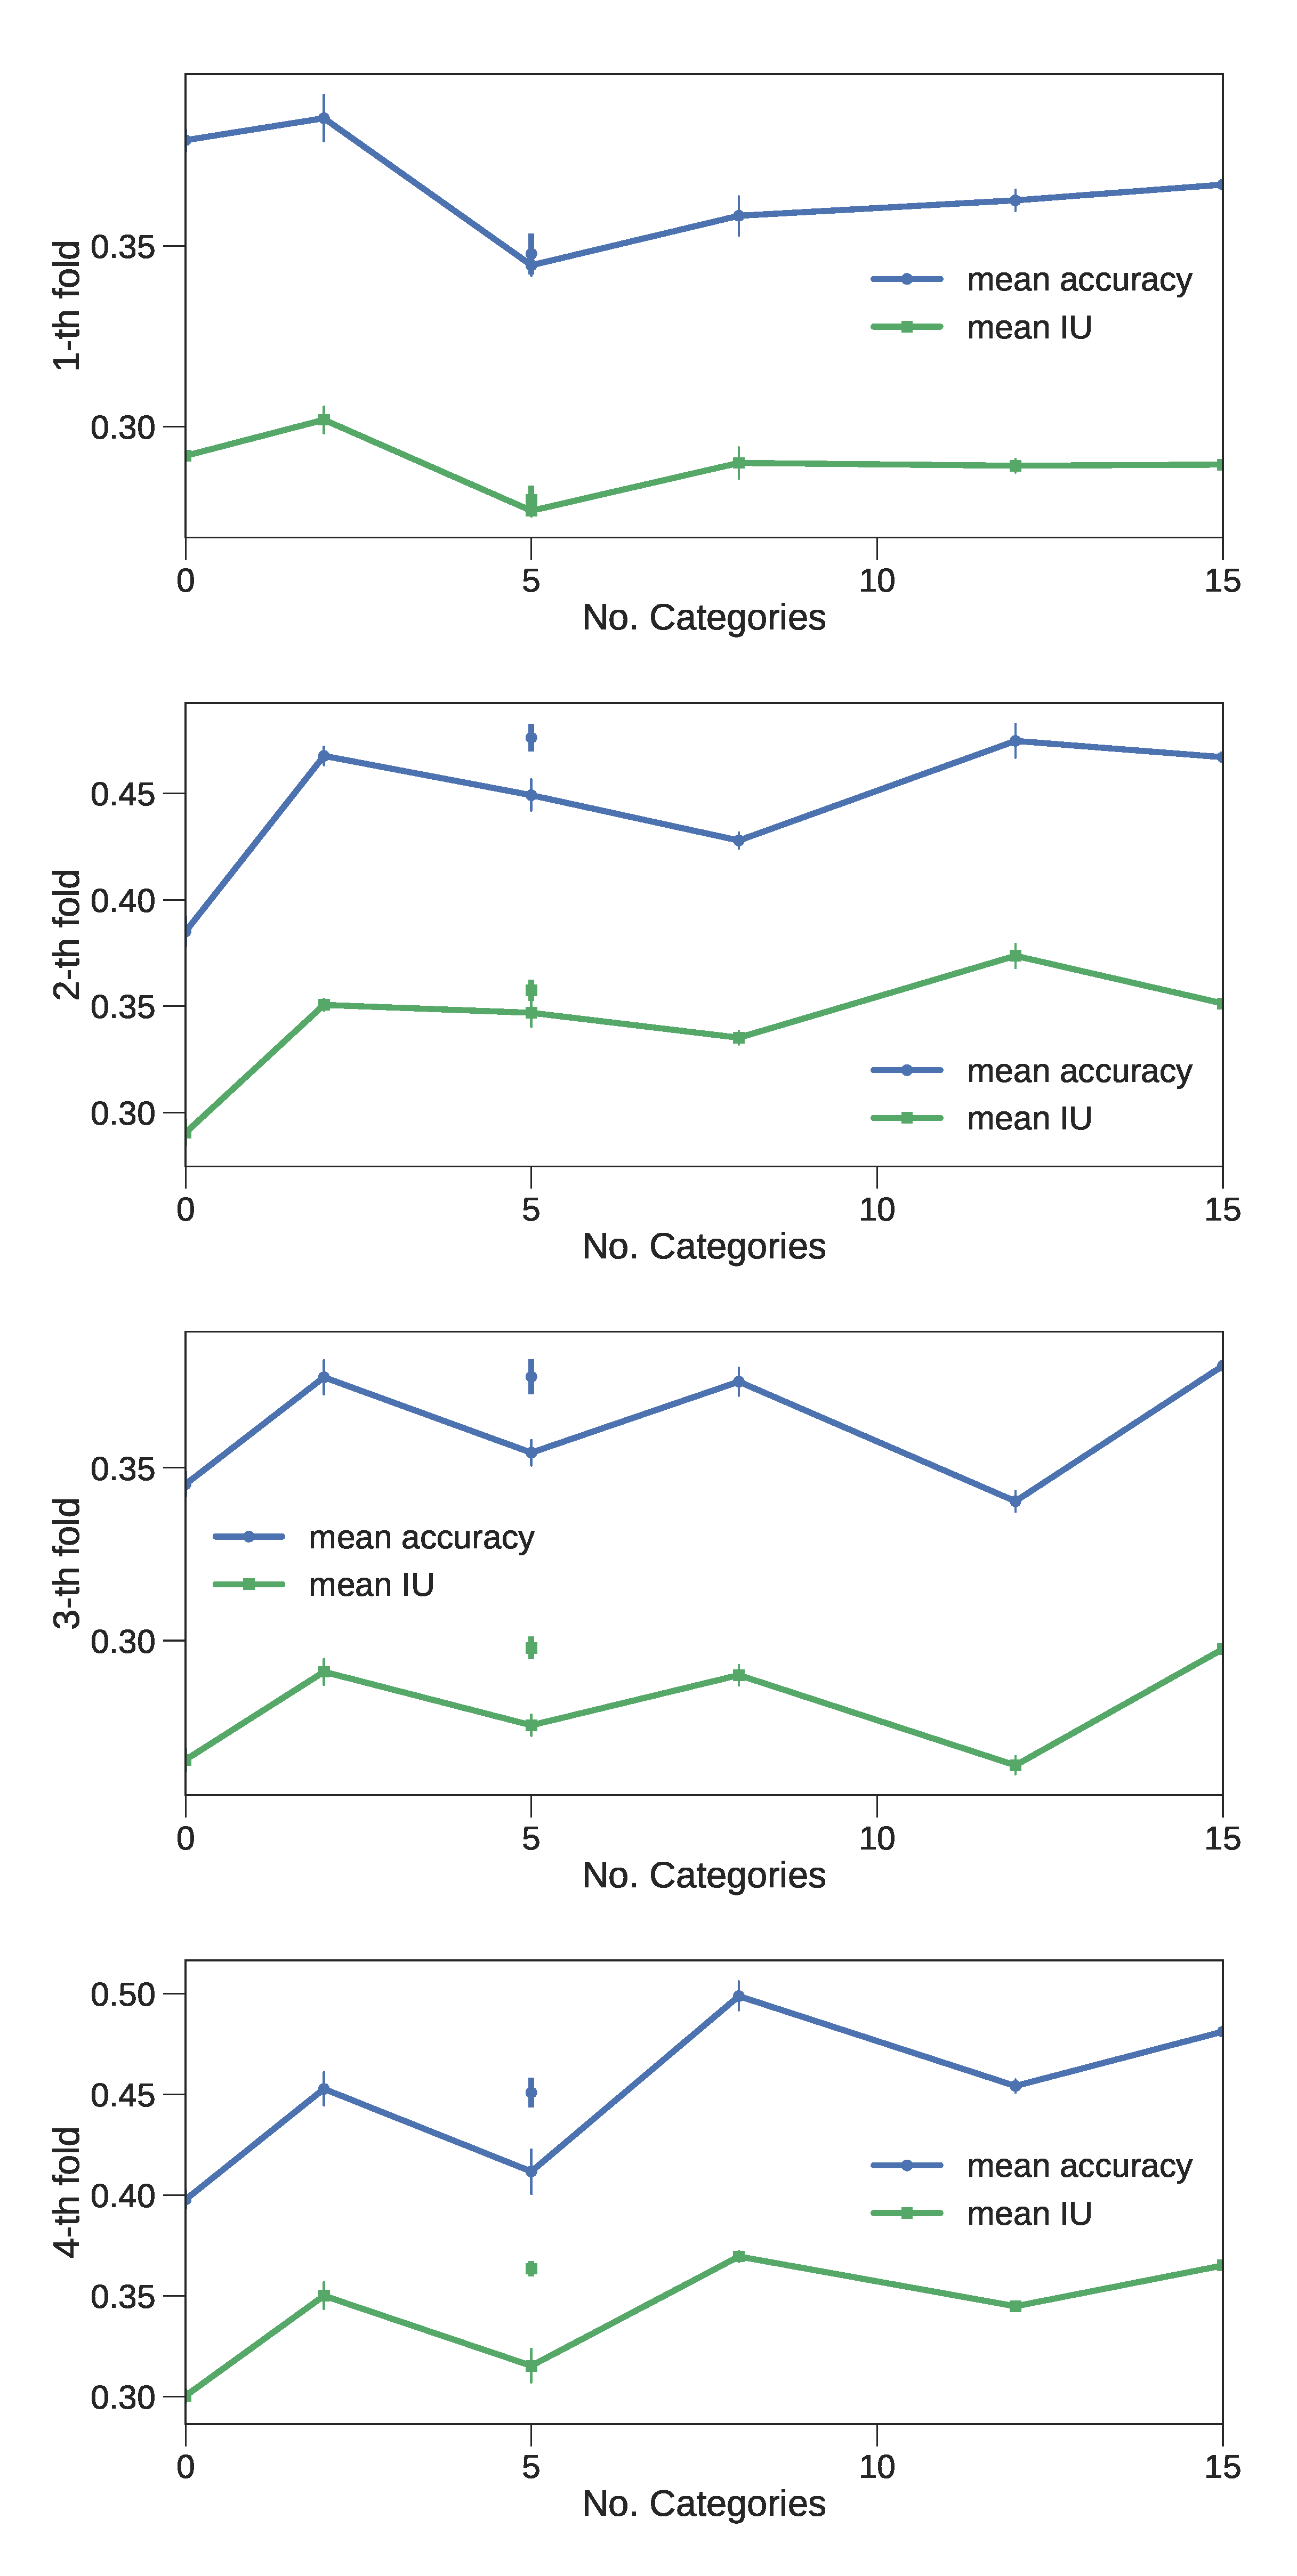
\includegraphics[width=\linewidth]{img/num_classes_folds.eps}
\caption{The influence of categorizing classes on test performance of fine-tuned models for each fold, addition to Figure \ref{fig:categories}.}
\label{fig:classesfold}
\end{figure}
